\chapter{The Basics of Maximum Likelihood Estimation \label{chapter:mlebasics}}

Beneath our discussions of classification, regression, and probability distributions in Chapters~\ref{chapter:classification}, \ref{chapter:regression}, and \ref{chapter:probabilitydistributions} lies the tricky problem of \textbf{model fitting}. We've seen what classification and regression models look like, but we still haven't addressed how to fit these models using training data.

Linear and logistic regression models are fit using a technique called \textbf{maximum likelihood (ML) estimation}, in which the model parameters are adjusted to maximize the joint probability of the observed data, or likelihood, given the model. 

For example, consider the five different datasets from Question~\ref{question:likexamples}. In each case, you have some data and an assumption about which probability distribution the data are drawn from. The job of maximum likelihood estimation is to use the data to identify the correct distributional parameters, such as $\mu$ and $\sigma$ (in the case of the normal distribution) or $\lambda$ (in the case of the Poisson distribution). This process is a type of \textbf{statistical inference}. 

\section{The Likelihood and Log-Likelihood}

Let $p(x|\theta)$ be the probability distribution that governs our data. Here, $\theta$ stands in for all of the parameters we want to fit. 

If we draw independent\footnote{Independent sampling just means that the values of different samples do not depend on each other. When the samples are drawn independently from the same distribution, their joint probability density is just the product of the individual probability densities (which are all the same).} samples from $p(x|\theta)$, the {\bf joint probability density function} for all $n$ observations is:
$$ p(x^{(1)}, x^{(2)}, \dots, x^{(n)}|\theta) = \prod_{i=1}^n p(x^{(i)}|\theta). $$
Since the data are known but the parameter(s) $\theta$ are unknown, we will view this quantity as a function of $\theta$. This is just a change in notation:
$$ \mathcal{L}(\theta) = \prod_{i=1}^n p(x^{(i)}|\theta). $$

The higher the joint probability of the data (the more ``likely'' the data are) given $\theta$, the higher the value of this function. We call $\mathcal{L}(\theta)$ the \textbf{likelihood}\footnote{The distributions we have discussed so far are from a broad family of probability distributions called the {\bf exponential family}. One of the properties of this family is that the log-likelihood is concave. Practically speaking, this means that if we maximize the log-likelihood by setting derivatives equal to zero, we are guaranteed to (a) get only one solution, and (b) find a maximum (not a minimum or an inflection point).}. Frequently we will want to work with the logarithm of the likelihood, which we call the \textbf{log-likelihood}, because it has some nice properties, including allowing us to manipulate sums instead of products\footnote{Note that if the function $f(z)$ has a maximum at $z'$, the function $\log f(z)$ will also have a maximum at $z'$, because the logarithmic function is monotonically increasing. So we will get the same parameter estimate(s) either way.}:
$$ \log \mathcal{L}(\theta) = \sum_{i=1}^n \log p(x^{(i)}|\theta). $$

In maximum likelihood estimation, we seek to find the $\theta$ for which the likelihood (or log-likelihood) is maximized. We do this by taking derivatives of the log-likelihood with respect to the various parameters and setting them equal to zero. The best-fit parameter estimates obtained in this way are called the \textbf{maximum likelihood estimates (MLEs)}. 
\vspace{5mm}

\begin{question}{}
What are some reasons why we might want to fit data to a probability distribution?
% Data summarization (don't need to keep entire dataset around)
% Sampling
% Many common models and hypothesis tests rely on parametric assumptions (T-tests, etc.)
% We are less likely to overfit to particularities of our own datasets, such as outliers (KNN, etc.)
% Detecting outliers or faulty assumptions
\end{question}

\section{Example: Fitting Data to a Normal Distribution}

Imagine you have some data from a lab test that measures the concentration of a particular biomarker. You have data from $100$ different subjects. A histogram of the raw data looks like this:
\begin{center}
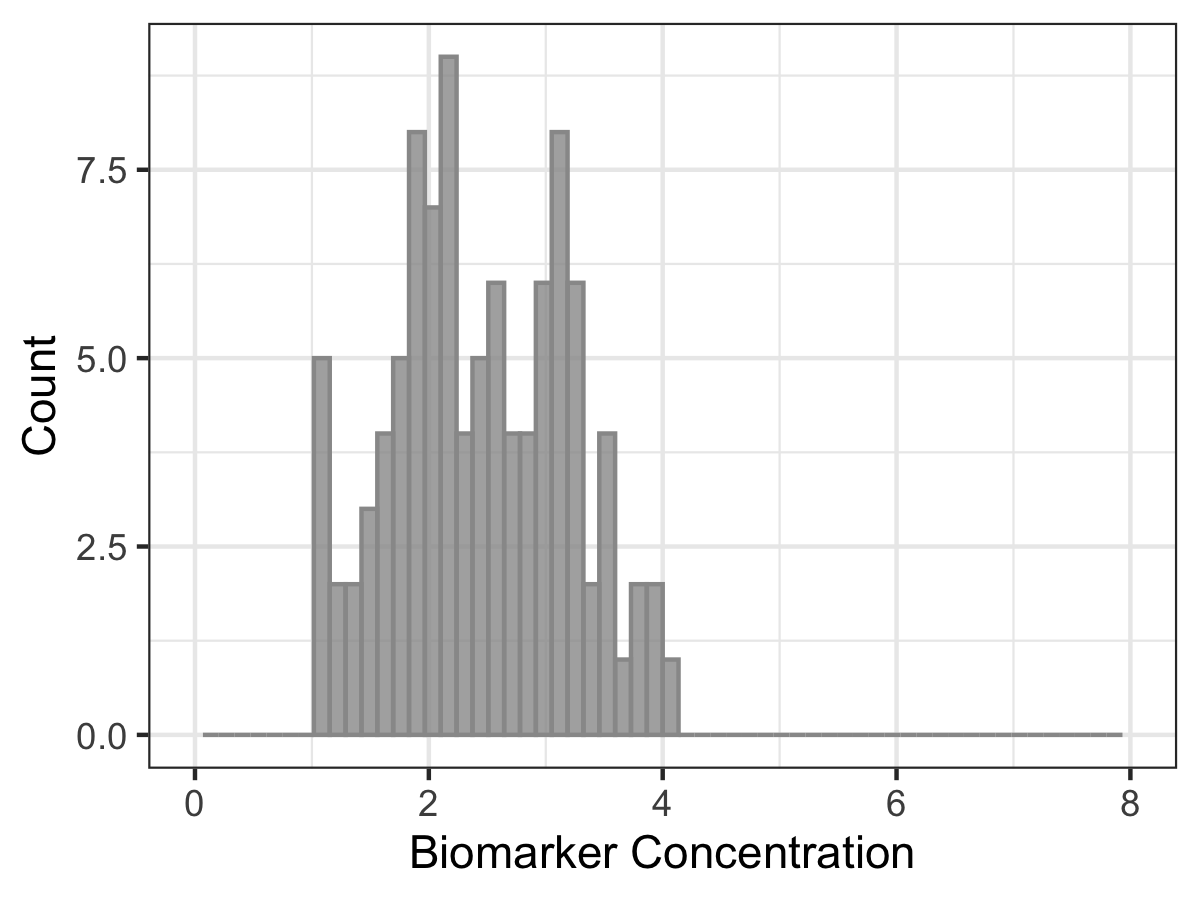
\includegraphics[width=0.7\textwidth]{img/normal-likelihood-example-data.png}
\end{center}

You want to find the normal distribution that best describes these data so you can create a reference distribution for this lab test. To do this, think about trying out several distributions with different values of $\mu$ and $\sigma$ and choosing the one that maximizes the log-likelihood. For example, here are three different normal distributions with different values of $\mu$ and $\sigma=0.7$: 
\begin{center}
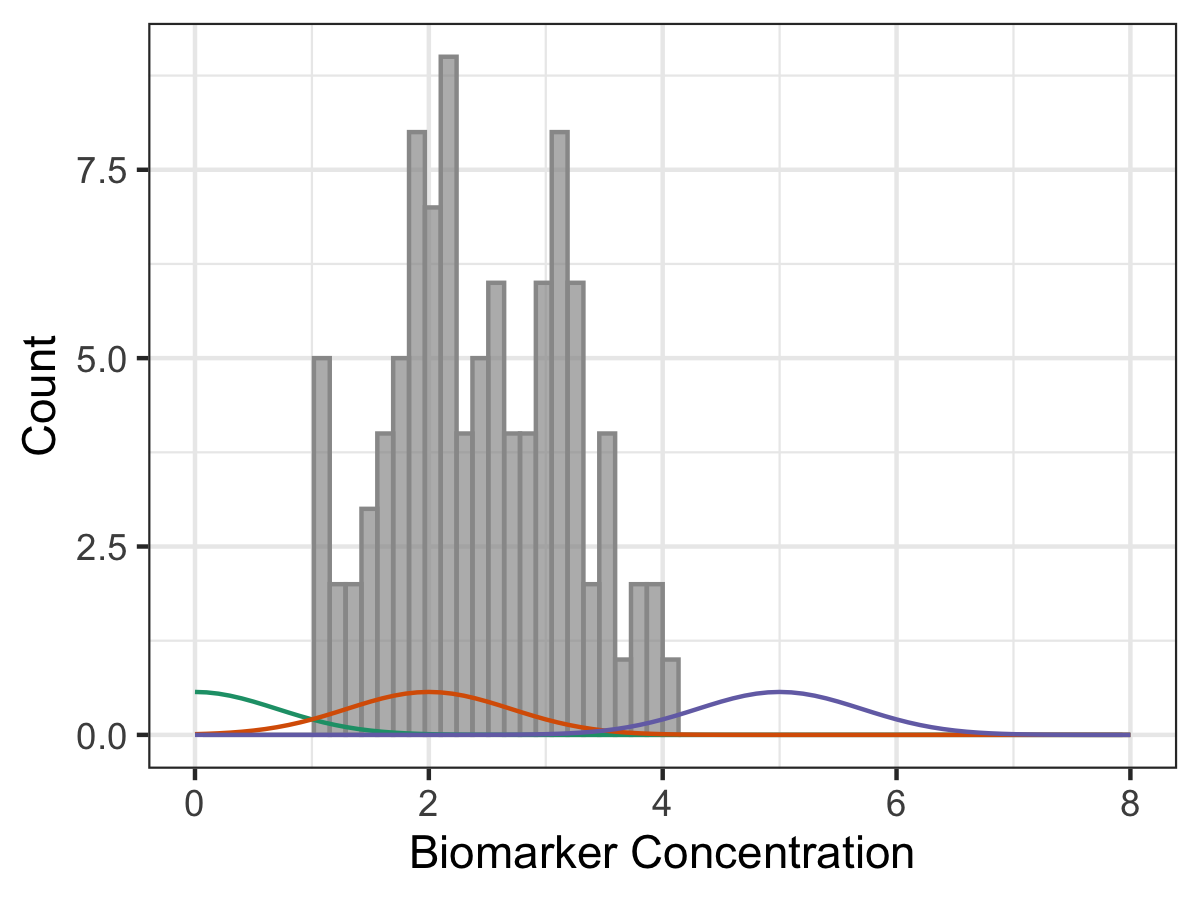
\includegraphics[width=0.7\textwidth]{img/normal-likelihood-example-data-normal.png}
\end{center}
Here is what happens to the log-likelihood as you vary $\mu$. The log-likelihoods of the three distributions shown in the plot above are shown as dots with their corresponding colors, and the maximum likelihood estimate is shown as a vertical dotted line.
\begin{center}
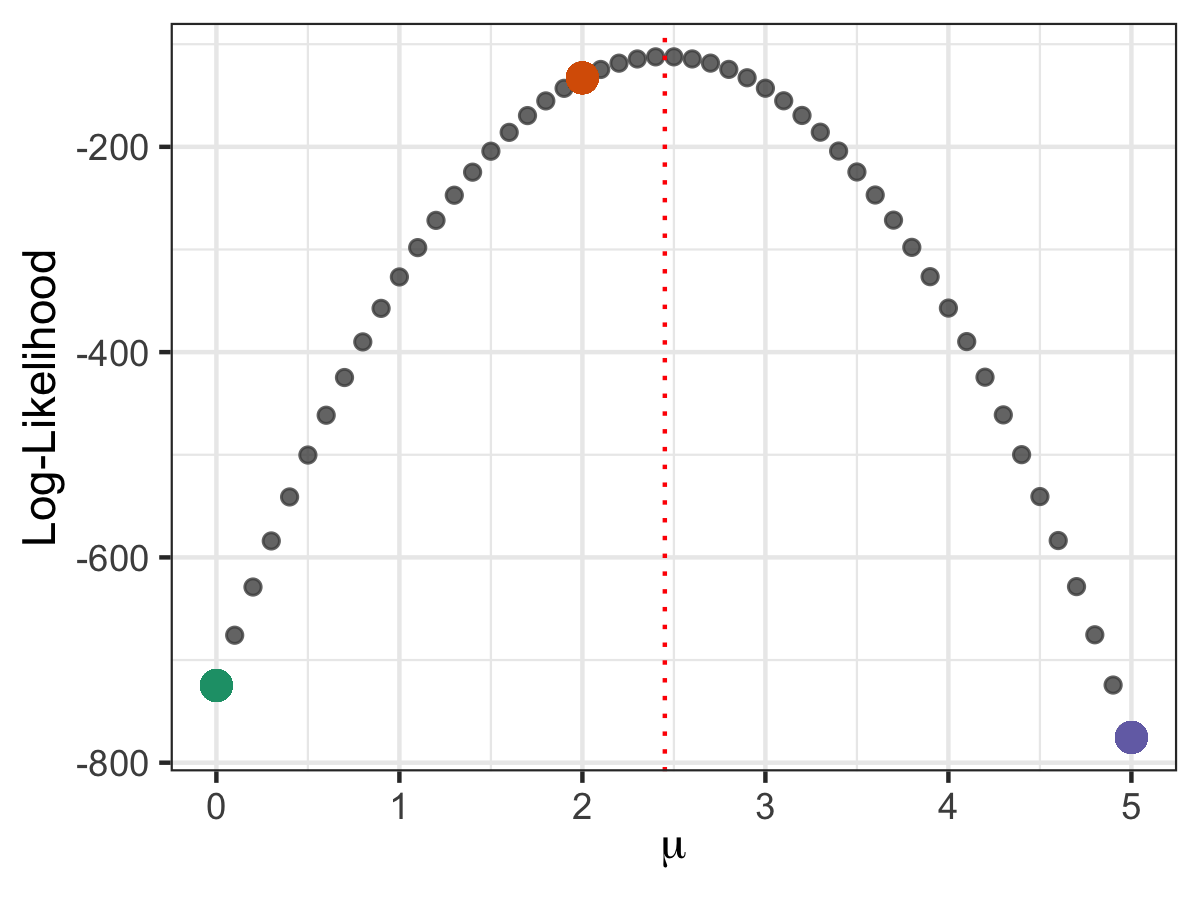
\includegraphics[width=0.7\textwidth]{img/normal-likelihood-example-vary-mu.png}
\end{center}
Now, here's what happens to the log-likelihood when we vary $\sigma$, keeping $\mu$ fixed at its maximum likelihood estimate from the graph above. Again, the maximum likelihood estimate is shown as a vertical dotted line. 
\begin{center}
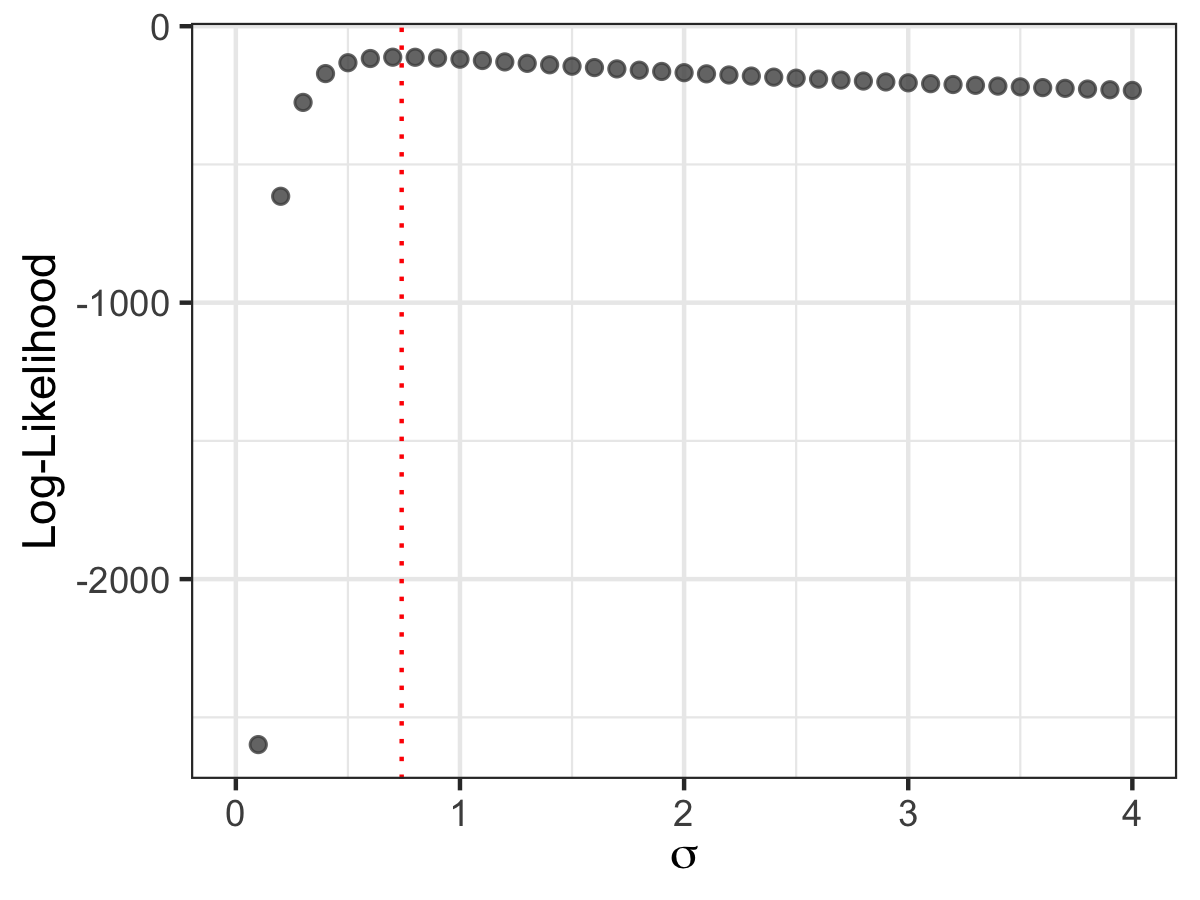
\includegraphics[width=0.7\textwidth]{img/normal-likelihood-example-vary-sigma.png}
\end{center}
For the record, I simulated these data from a normal distribution with $\mu=2.5$ and $\sigma=0.75$. The maximum likelihood estimates obtained from this dataset are $\hat{\mu} = 2.45$ and $\hat{\sigma} = 0.74$. 

\section{Analytical Calculations of MLEs}

In some simple cases, the MLEs can be calculated analytically. We will now go through a bunch of examples of how to find the MLEs of the probability distributions we saw in Chapter~\ref{chapter:probabilitydistributions}. 

\subsection{Bernoulli Distribution}

The Bernoulli distribution is described in Section~\ref{sect:bernoulli}. Our goal is to find the parameter, $\mu$, of this distribution, given some observed data, $x^{(1)}, \dots, x^{(n)}$. The data will consist of a list of 1s and 0s, since Bernoulli random variables can only take the values 0 or 1.

To find $\hat{\mu}$, our MLE for $\mu$, we first write down the log-likelihood:
\begin{align*}
\log \mathcal{L}(\mu) &= \sum_{i=1}^n \log p(x^{(i)}|\mu) \\
&= \sum_{i=1}^n \log \left( \mu^{x^{(i)}}(1-\mu)^{1-x^{(i)}} \right) \\
&= \sum_{i=1}^n \left[ x^{(i)} \log(\mu) + (1-x^{(i)}) \log(1-\mu) \right] \end{align*}
Then we take the derivative of the log-likelihood with respect to $\mu$:
\begin{align*}
\frac{d}{d \mu} \log \mathcal{L}(\mu) = \sum_{i=1}^n \left[ \frac{x^{(i)}}{\mu} - \frac{1-x^{(i)}}{1-\mu} \right]
\end{align*}
The MLE of $\mu$ will occur when the likelihood is maximized, which happens when the first derivative equals zero. So to solve for $\hat{\mu}$, we set the derivative equal to zero and rearrange:
\begin{align*} \sum_{i=1}^n \left[ \frac{x^{(i)}}{\hat{\mu}} - \frac{1-x^{(i)}}{1-\hat{\mu}} \right] = 0 & \implies (1 - \hat{\mu}) \sum_{i=1}^n x^{(i)} = \hat{\mu} \sum_{i=1}^n (1 - x^{(i)}) \\
& \implies \boxed{\hat{\mu} = \frac{1}{n} \sum_{i=1}^n x^{(i)}} \end{align*}
We see that the MLE, $\hat{\mu}$, is simply the sum of our data -- i.e. the number of data points where the outcome is 1 -- divided by the total number of observations. 

This makes sense: if you want to know the probability that a coin will come up heads, a good way to estimate it is to flip the coin a bunch of times and calculate the fraction of observations in which the coin comes up heads. 

\subsection{Binomial Distribution}

The binomial distribution is described in Section~\ref{sect:binomial}. We will make one notational change from that section, which is to call the number of Bernoulli trials $m$ instead of $n$, since we are using $n$ to refer to the number of data samples. To keep things simple, we will assume that $m$ is a known quantity. As before, we first write down the log-likelihood:
\begin{align*}
\log \mathcal{L}(\mu) &= \sum_{i=1}^n \log p(x^{(i)}|m,\mu) \\
&= \sum_{i=1}^n \log \left[ {m\choose x} \mu^x (1 - \mu) ^ {m-x} \right] \\
&= \sum_{i=1}^n \left[\log(m!) - \log(x!) - \log((m-x)!) + x^{(i)} \log(\mu) + (m-x^{(i)}) \log(1-\mu) \right] \end{align*}
Then we take the derivative of the log-likelihood with respect to $\mu$:
\begin{align*}
\frac{d}{d \mu} \log \mathcal{L}(\mu) = \sum_{i=1}^n \left[ \frac{x^{(i)}}{\mu} - \frac{m-x^{(i)}}{1-\mu} \right]
\end{align*}
We set this equal to zero and solve for $\hat{\mu}$ (the maximum likelihood estimate of $\mu$):
\begin{align*} \sum_{i=1}^n \left[ \frac{x^{(i)}}{\hat{\mu}} - \frac{m-x^{(i)}}{1-\hat{\mu}} \right] = 0 & \implies (1 - \hat{\mu}) \sum_{i=1}^n x^{(i)} = \hat{\mu} \sum_{i=1}^n (m - x^{(i)}) \\
& \implies \boxed{\hat{\mu} = \frac{1}{nm} \sum_{i=1}^n x^{(i)}} \end{align*}

\begin{question}{}
Interpret the MLE for the parameter, $\mu$, of a binomial distribution, assuming fixed $m$ (number of trials). Does the MLE for $\mu$ make intuitive sense to you? Think through a few of your examples from Question~\ref{question:binomialex}. 
\end{question}

\subsection{Normal Distribution \label{sect:mlenormal}}

The normal distribution is described in Section~\ref{sect:normal}. We will follow the same procedure as in the previous two sections, except that now we have two parameters to solve for, $\mu$ and $\sigma$, instead of one. First, we write down the log-likelihood:
\begin{align*}
\log \mathcal{L}(\mu, \sigma) &= \sum_{i=1}^n \log p(x^{(i)}|\mu, \sigma) \\
&= \sum_{i=1}^n \log \left( \frac{1}{\sqrt{2 \pi \sigma^2}} e^{-\frac{(x^{(i)}-\mu)^2}{2 \sigma^2}} \right) \\
&= -\frac{n}{2} \log (2 \pi) - \frac{n}{2} \log \sigma^2 - \frac{1}{2 \sigma^2} \sum_{i=1}^n \left( x^{(i)} - \mu \right)^2 \\
\end{align*}
To find the MLE for $\mu$, we take the derivative of the log-likelihood with respect to $\mu$:
\begin{align*}
\frac{\partial}{\partial \mu} \log \mathcal{L}(\mu, \sigma) = \frac{1}{\sigma^2} \sum_{i=1}^n \left( x^{(i)} - \mu \right)
\end{align*}
We set this equal to zero and solve for $\hat{\mu}$ (the maximum likelihood estimate of $\mu$):
\begin{align*} \frac{1}{\sigma^2} \sum_{i=1}^n \left( x^{(i)} - \mu \right) = 0 & \implies \boxed{\hat{\mu} = \frac{1}{n} \sum_{i=1}^n x^{(i)}} \end{align*}
To find the MLE for $\sigma$, we then take the derivative of the log-likelihood with respect to $\sigma$:
\begin{align*} \frac{\partial}{\partial \sigma} \log \mathcal{L}(\mu, \sigma) &= -\frac{n}{\sigma} + \frac{1}{\sigma^3} \sum_{i=1}^n \left( x^{(i)} - \mu \right)^2
\end{align*}
We set this equal to zero and solve for $\hat{\sigma}$ (the maximum likelihood estimate of $\sigma$)\footnote{One detail: it turns out this estimate is biased because it depends on the MLE for $\mu$. An unbiased version has $n-1$ in the denominator instead of $n$. The effect of this is minimal unless $n$ is small.}. Note that the answer depends on our previously calculated MLE for $\mu$:
\begin{align*}
-\frac{n}{\hat{\sigma}} + \frac{1}{\hat{\sigma}^3} \sum_{i=1}^n \left( x^{(i)} - \mu \right)^2 = 0  & \implies \boxed{\hat{\sigma} = \sqrt{\frac{1}{n} \sum_{i=1}^n \left( x^{(i)} - \hat{\mu} \right)^2}}
\end{align*}

\begin{question}{}
Interpret the MLEs for the parameters, $\mu$ and $\sigma$, of a normal distribution. Do these results make intuitive sense to you? Think through a few of your examples from Question~\ref{question:normalex}. 
\end{question}

\subsection{Poisson Distribution}

The Poisson distribution is described in Section~\ref{sect:poisson}. To find the MLE for $\lambda$, its mean, we first (as usual) write down the log-likelihood:
\begin{align*}
\log \mathcal{L}(\lambda) &= \sum_{i=1}^n \log p(x^{(i)}|\lambda) \\
&= \sum_{i=1}^n \log \left( \frac{e^{-\lambda} \lambda^{x^{(i)}}}{x^{(i)}!} \right) \\
&= \sum_{i=1}^n \left[ -\lambda + x^{(i)} \log(\lambda) - \log(x^{(i)}!) \right] \end{align*}
Now we take the derivative of the log-likelihood with respect to $\lambda$:
\begin{align*}
\frac{d}{d \lambda} \log \mathcal{L}(\lambda) = \sum_{i=1}^n \left[ -1 + \frac{x^{(i)}}{\lambda} \right]
\end{align*}
We set this equal to zero and solve for $\hat{\lambda}$ (the maximum likelihood estimate of $\lambda$):
\begin{align*} \sum_{i=1}^n \left[ -1 + \frac{x^{(i)}}{\hat{\lambda}} \right] = 0 & \implies \boxed{\hat{\lambda} = \frac{1}{n} \sum_{i=1}^n x^{(i)}} \end{align*}

\begin{question}{}
Interpret the MLE for the parameter, $\lambda$, of a Poisson distribution. Does this result make intuitive sense to you? Think through a few of your examples from Question~\ref{question:poissonex}. 
\end{question}

\subsection{Geometric Distribution}

The geometric distribution is described in Section~\ref{sect:geometric}. To find the MLE for $\mu$, we first write down the log-likelihood:
\begin{align*}
\log \mathcal{L}(\mu) &= \sum_{i=1}^n \log p(x^{(i)}|\mu) \\
&= \sum_{i=1}^n \log \left( (1-\mu)^{x^{(i)}} \mu \right) \\
&= \sum_{i=1}^n \left[ x^{(i)} \log(1-\mu) + \log(\mu) \right] \end{align*}
Now we take the derivative of the log-likelihood with respect to $\mu$:
\begin{align*}
\frac{d}{d \mu} \log \mathcal{L}(\mu) = \sum_{i=1}^n \left[ -\frac{x^{(i)}}{1-\mu} + \frac{1}{\mu} \right]
\end{align*}
We set this equal to zero and solve for $\hat{\mu}$ (the maximum likelihood estimate of $\mu$):
\begin{align*} \sum_{i=1}^n \left[ -\frac{x^{(i)}}{1-\hat{\mu}} + \frac{1}{\hat{\mu}} \right] = 0 & \implies \frac{n}{\hat{\mu}} = \frac{1}{1 - \hat{\mu}} \sum_{i=1}^n x^{(i)} \\
& \implies \boxed{\hat{\mu} = \frac{n}{\sum_{i=1}^n (x^{(i)}+1)} }\end{align*}

\begin{question}{}
Interpret the MLE for the parameter, $\mu$, of a geometric distribution. Does this result make intuitive sense to you? Think through a few of your examples from Question~\ref{question:geometricex}. 
\end{question}

\subsection{Exponential Distribution}

The exponential distribution is described in Section~\ref{sect:exponential}. To find the MLE for $\lambda$, we first write down the log-likelihood:
\begin{align*}
\log \mathcal{L}(\lambda) &= \sum_{i=1}^n \log p(x^{(i)}|\lambda) \\
&= \sum_{i=1}^n \log \left( \lambda e^{-\lambda x^{(i)}} \right) \\
&= \sum_{i=1}^n \left[\log(\lambda) - \lambda x^{(i)} \right] \end{align*}
Now we take the derivative of the log-likelihood with respect to $\lambda$:
\begin{align*}
\frac{d}{d \lambda} \log \mathcal{L}(\lambda) = \sum_{i=1}^n \left[ \frac{1}{\lambda} - x^{(i)} \right]
\end{align*}
We set this equal to zero and solve for $\hat{\lambda}$ (the maximum likelihood estimate of $\lambda$):
\begin{align*} \sum_{i=1}^n \left[ \frac{1}{\hat{\lambda}} - x^{(i)} \right] = 0 & \implies \boxed{\hat{\lambda} = \frac{n}{\sum_{i=1}^n x^{(i)}}} \end{align*}

\begin{question}{}
Interpret the MLE for the parameter, $\lambda$, of an exponential distribution. Does this result make intuitive sense to you? Think through a few of your examples from Question~\ref{question:exponentialex}. 
\end{question}

\section{Summary of MLEs for Common Distributions}

The table below contains a summary of the MLEs of various parameters from some common probability distributions.

\begin{center} {\small
\begin{tabular}{lccc}
\toprule
Distribution & Parameter & ML Estimate & Domain of $x^{(i)}$ \\
\midrule
Univariate Normal & $\mu$ & $\displaystyle \cfrac{1}{n} \sum_{i=1}^n x^{(i)}$  & $\mathbb{R}$ \\
& $\sigma$ & $\displaystyle \frac{1}{n} \sum_{i=1}^n \left(x^{(i)} - \hat{\mu}\right)^2 $ & $\mathbb{R}$ \\
Multivariate Normal & $\mu$ & $\displaystyle \frac{1}{n} \sum_{i=1}^n x^{(i)}$ & $\mathbb{R}^m$ \\
& $\boldsymbol\Sigma$ & $\displaystyle \frac{1}{n} \sum_{i=1}^n (x^{(i)}-\hat{\mu})(x^{(i)}-\hat{\mu})^T$ & $\mathbb{R}^m$ \\
Bernoulli & $\mu$ & $\displaystyle \frac{1}{n} \sum_{i=1}^n x^{(i)}$ & $\{0, 1\}$ \\
Binomial (fixed $m$) & $\mu$ & $\displaystyle \frac{1}{nm} \sum_{i=1}^n x^{(i)}$ & $\left\{ 0, 1, \dots, m \right\}$ \\
Poisson & $\lambda$ & $\displaystyle \frac{1}{n} \sum_{i=1}^n x^{(i)}$ & $\left\{ 0, 1, \dots \right\}$\\
Geometric & $\mu$ & $\displaystyle \cfrac{n}{\sum_{i=1}^n (x^{(i)} + 1)} $ & $\left\{ 0, 1, \dots \right\}$ \\
Exponential & $\lambda$ & $\displaystyle \cfrac{n}{\sum_{i=1}^n x^{(i)}} $ & $\mathbb{R}^+$ \\
\bottomrule
\end{tabular}}
\end{center}

\begin{question}{}
In Question~\ref{question:likexamples}, we examined several examples of experimental conditions and datasets and discussed which probability distribution best modeled each one. Using the formulas above and the actual datasets from Question~\ref{question:likexamples}, calculate the MLEs for the parameter(s) of your chosen probability distributions. 
\end{question}
